\subsection{Описание данных}
\par
Рассматриваемый набор данных (скважина T1) содержит показания двух типов датчиков: распределенного термоанемометра – шесть одинаковых ТА датчиков, равномерно расположенных по азимуту на окружности в сечении скважины, и вспомогательного датчика, измеряющего фоновую температуру в центре окружности на оси прибора.

\subsubsection{Осевой датчик фоновой температуры}
\par
Фоновая температура в центре скважины измерена скважинным прибором PLT-9.2, который включает в себя датчик температуры со следующими характеристиками \cite{92}:

\begin{center}
\begin{tabular}{ |c|c| } 
 \hline
 Диапазон измерения температуры, $\degree C$ & от 0 до +120(150) \\ 
 \hline
 Основная погрешность измерения температуры, $\degree C$ & 1 \\ 
 \hline
 Разрешающая способность измерения температуры, $\degree C$ & 0.001 \\ 
 \hline
 Тепловая инерция измерения температуры, сек. & 1 \\
 \hline
\end{tabular}
\end{center}

\par
В исследуемом наборе данных температура записана с нерегулярно меняющимся шагом по времени от $\Delta t_{min}=0.7$ сек. до $\Delta t_{max}=4.1$ сек со средним значением $\Delta t_{avg}=1.8\pm0.6$ сек и фиксированным шагом по пространству $\Delta x=0.1$м.
\par
Разброс значений температуры лежит в интервале от $T_{min}=27.6\degree C$ до $T_{max}=28.5\degree C$ со средним значением $T_{avg}=28.3\pm0.2\degree C$.

\subsubsection{Азимутально распределенный термоанемометр}
\par
Прибор PLT-0.6.3 включает в себя шесть азимутально расположенных термоанемометров. Каждый из этих датчиков работает в цикле нагревания-охлаждения: нагревается 4 секунды и охлаждается 8 секунды. Датчики нагреваются и охлаждаются попарно – пара составляется противоположными по азимуту датчиками. Другими словами, если пронумеровать датчики по кругу номерами $i=1,..,6$, то общий циклический процесс начиная с произвольного момента времени $t=t_0$ может выглядеть так:
\begin{enumerate}[label=\arabic*.]
    \item $t_0 \leq t < t_0+4c$ : датчики 1 и 4 нагреваются; датчики 2, 3, 5, 6 охлаждаются.
    \item $t_0+4c \leq t < t_0+8c$ : датчики 2 и 5 нагреваются; датчики 1, 3, 4, 6 охлаждаются.
    \item $t_0+8c \leq t < t_0+12c$ : датчики 3 и 6 нагреваются; датчики 1, 2, 4, 5 охлаждаются.
    \item $t_0+12c \leq t < t_0+16c$ : датчики 1 и 4 нагреваются; датчики 2, 3, 5, 6 охлаждаются, 
\end{enumerate}
И так далее.
\par
Запись измерений температуры происходит каждую 0.1 секунды, что дает 120 точек на каждый цикл нагревания-охлаждения. Пример пяти последовательно измеренных циклов нагревания-охлаждения показан на рис.\ref{fig:cycle_examples}.

\newpage
\begin{figure}[H]
\centering
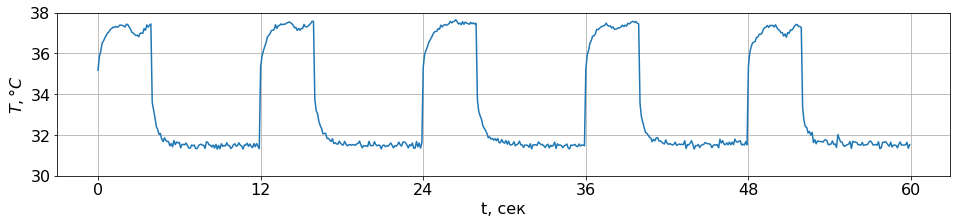
\includegraphics[width=1.0\textwidth]{TA/cycle_examples.png}
\caption{Пример пять последовательно расположенных циклов нагревания-охлаждения.}
\label{fig:cycle_examples}
\end{figure}


\subsection{Формулировка задачи}
\subsubsection{Физическая постановка задачи}
\par
Прибор движется по скважине; погруженные во флюид датчики нагреваются и охлаждаются. Характер поведения циклов нагревания-охлаждения зависит от типа флюида и его скорости относительно датчика.  
\par
Датчики термоанемометрии достаточно точные, чтобы можно было пренебречь тепловой инерцией и считать все показания измеренными с хорошей точностью; это неприменимо к осевой температуре, которая измеряется гораздо менее точным датчиком. Поэтому осевую температуру необходимо скорректировать с учетом характеристик прибора.
\par
По данным обоих приборов необходимо в общей постановке задачи определить скорость и фазовый состав протекающего через каждый датчик флюида. В данной работе опускается задача вычисления скорости флюидов, в существующих исследованиях выполняющаяся на основе корреляции признаков циклов нагревания-охлаждения с лабораторными данными. 
\par
Рассматривается задача определения фазового состава для каждого цикла. Так как скважина горизонтальная, в произвольный момент времени некоторые из шести датчиков могут находиться в разных фазах, поэтому анализ каждого датчика необходимо проводить отдельно. Отметим, что прибор может непроизвольно вращаться вокруг своей оси, продвигаясь вдоль скважины.

\subsubsection{Математическая постановка задачи}
\par
В качестве датасета рассматривается множество последовательно измеренных одним датчиком циклов нагревания-охлаждения. Под циклом понимается 120 значений температуры, измеренных с шагом 0.1 сек на некотором промежутке глубины вдоль скважины, и соответствующие этому интервалу глубины одно или несколько значений фоновой осевой температуры. Рассматривается шесть датасетов, соответствующие показаниям шести датчиков; в каждом датасете содержится около 1500 циклов.
\par
Используя доступные данные, для каждого цикла в каждом датасете необходимо предсказать метку: либо одна определенная фаза (вода, нефть, газ), либо смешанная фаза с оценкой фазового состава (например, 70\% воды и 30\% нефти).